        \clearpage
        \begin{figure*}[ht]
            \pdfbookmark[2]{ID 03}{figure_id_03}
        	\centering
            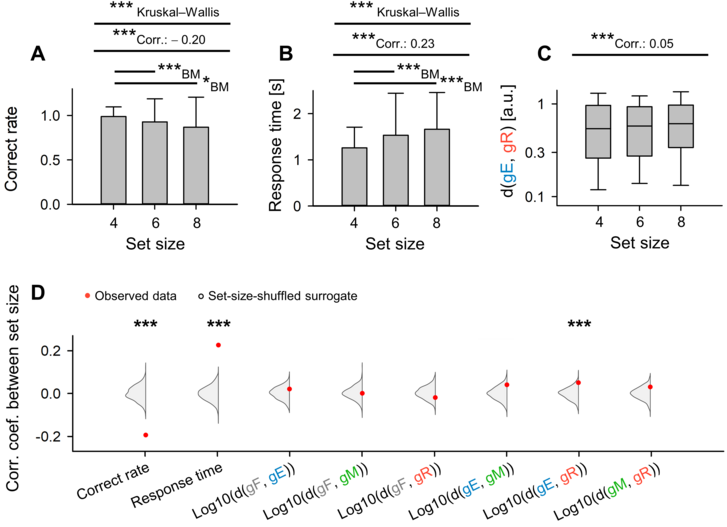
\includegraphics[width=1\textwidth]{./media/figures/.png/Figure_ID_03.png}
        	\caption{\textbf{
Influence of memory load on encoding and retrieval states in the hippocampus
}
\smallskip
\\
\textbf{\textit{A.}} Relationship between set size (number of letters encoded) and correct rate in the WM task. Notably, a negative correlation was observed (coefficient = $-$ 0.20, ***\textit{p} $<$ 0.001), analyzed using set-size-shuffled surrogate. Significance was determined using Kruskal--Wallis test, followed by the Brunner--Munzel test with Bonferroni correction. \textbf{\textit{B.}}  Association between set size and response time post-probe initiation. A positive correlation was detected (coefficient = 0.23, ***\textit{p} $<$ 0.001), analyzed using set-size-shuffled surrogate. Statistical tests included the Kruskal--Wallis and post-hoc Brunner--Munzel tests with Bonferroni correction. \textbf{\textit{C.}}  Analysis of set size against the distance between geometric medians during encoding and retrieval phases (represented as $\lVert \mathrm{g_{E}g_{R}} \rVert$). A correlation of 0.05 was noted for set size and $\mathrm{log_{10}{\lVert g_{E}g_{R} \rVert}}$), analyzed using set-size-shuffled surrogate. \textbf{\textit{D.}}  Experimentally observed correlations between set size and various parameters are illustrated by \textit{red} dots. The \textit{gray} violin plots contrast these findings with set-size-shuffled surrogate data (\textit{n} = 1,000), emphasizing the significant observed correlation coefficients (***\textit{p} $<$ 0.001). Abbreviations: $\mathrm{g_{F}}$, $\mathrm{g_{E}}$, $\mathrm{g_{M}}$, $\mathrm{g_{R}}$ represent the geometric median of trajectories during fixation, encoding, maintenance, and retrieval phases, respectively.
}
% width=1\textwidth
        	\label{fig:03}
        \end{figure*}
